\documentclass[10pt,a4paper]{article}
\usepackage[margin=17mm]{geometry}
\usepackage{fontspec}
\setmainfont{TeX Gyre Termes}
\usepackage{amsmath,graphicx,xcolor}
\definecolor{ink}{HTML}{173C58}
\pagestyle{empty}
\setlength{\parindent}{0pt}
\setlength{\parskip}{5pt}
\begin{document}
\begin{center}
{\Large\bfseries\color{ink} AIAA3201 Lab Week 07}\\[3pt]
{\normalsize CNN Optimization, Regularization, and Transfer Learning}
\end{center}
\vspace{-5pt}

\textbf{1. Activation functions.}
The elementwise sigmoid $\sigma(x)=1/(1+e^{-x})$ maps inputs to $(0,1)$. Its backward pass follows the chain rule: $dx=dout\,\sigma(x)(1-\sigma(x))$, so the upstream gradient must be included. ReLU computes $\max(0,x)$, retaining positive activations and suppressing negative ones. NumPy operations vectorize these calculations over arbitrary array shapes without explicit element loops.

\textbf{2. Momentum and Adam: why bias correction is needed.}
Momentum accumulates $v_t=\rho v_{t-1}+g_t$ and updates $w_t=w_{t-1}-\eta v_t$, smoothing changing gradient directions. Adam maintains $m_t=\beta_1m_{t-1}+(1-\beta_1)g_t$ and $v_t=\beta_2v_{t-1}+(1-\beta_2)g_t^2$. Starting both estimates at zero biases them toward zero early in training: under stationary moments, $E[m_t]=(1-\beta_1^t)E[g_t]$ and $E[v_t]=(1-\beta_2^t)E[g_t^2]$. The corrections
\[
\widehat m_t=\frac{m_t}{1-\beta_1^t},\qquad
\widehat v_t=\frac{v_t}{1-\beta_2^t},\qquad
w_t=w_{t-1}-\eta\frac{\widehat m_t}{\sqrt{\widehat v_t}+\epsilon}
\]
remove this initialization bias. The two factors differ and do not generally cancel in the update; omitting them distorts early step sizes. The returned states remain the uncorrected $m_t,v_t$ for the next iteration.

\textbf{3. Inverted dropout: training scaling and test identity.}
Here $p$ is the probability of \emph{keeping} an activation. For an independent mask $b\sim\mathrm{Bernoulli}(p)$, training returns $y=xb/p$. Because $E[b/p]=1$, $E[y\mid x]=x$; without the factor $1/p$, the expectation would be $px$. Random removal discourages reliance on particular other units. At test time all activations are retained and the input is returned unchanged: training already compensated for the expected removal, so further scaling would change the activation scale. This preserves layerwise expectations, not exact equality between a nonlinear network and an ensemble of dropout networks.

\textbf{4. Batch normalization.}
Training computes each feature's batch mean $\mu_B$ and population variance $s_B^2$ along axis 0, then applies $y=\gamma(x-\mu_B)/\sqrt{s_B^2+\epsilon}+\beta$. The learned affine terms retain representational flexibility, and $\epsilon$ protects constant features from division by zero. Each running statistic is updated as $r\leftarrow\mathrm{momentum}\,r+(1-\mathrm{momentum})r_B$. Testing uses only these stored statistics and leaves them unchanged, avoiding dependence on the current test batch, including when it contains a single example.

\textbf{5. Transfer learning.}
ResNet18 is loaded with \texttt{ResNet18\_Weights.DEFAULT} to reuse pretrained ImageNet features. All original parameters are frozen; \texttt{model.fc} is then replaced with a linear layer mapping its existing input dimension to the requested class count. The new head is trainable by default. This adapts the classifier while retaining backbone weights; parameter freezing alone does not stop BatchNorm running-buffer updates in training mode. Evaluation mode is used for the supplemental inference checks.

\textbf{Verification.}
The unchanged official script produced all 10 check marks below. The image reproduces its captured check lines in two columns; full stdout and stderr are retained separately. Five supplemental check groups passed: sigmoid finite differences with non-unit upstream gradients; five Adam steps against PyTorch; dropout at $p=0.2,0.7,1$; BatchNorm affine/momentum/constant-feature and fixed-statistic checks; and ResNet18 output shapes plus freezing for 3 and 7 classes.

\begin{center}
\vspace{-3pt}
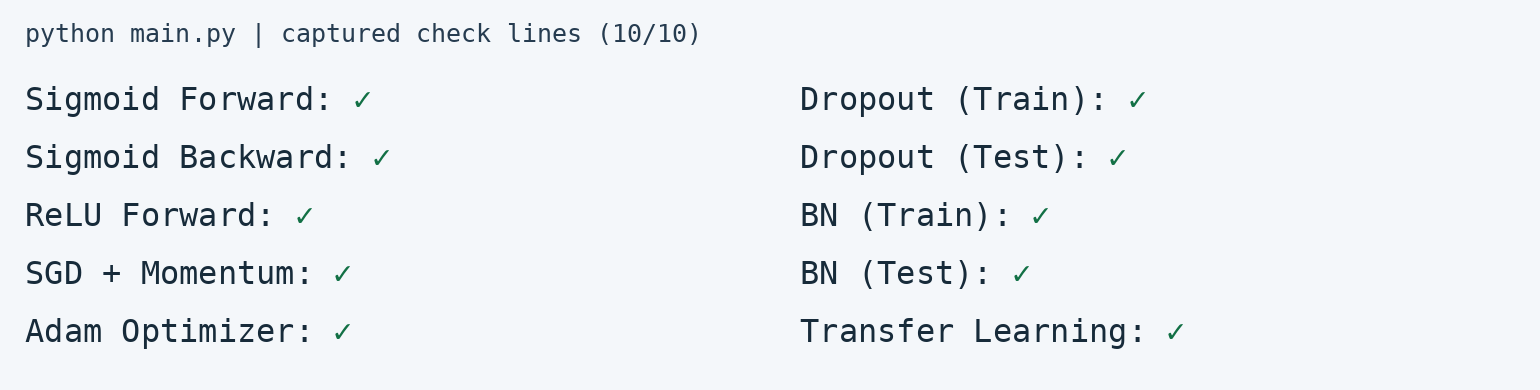
\includegraphics[width=\linewidth]{screenshots/verification.png}
\end{center}
\vspace{-9pt}
{\footnotesize Implementation: only the supplied code blocks were filled; original comments and the verification script were preserved.}
\end{document}
